% Pôster A1 — Mineração de Regras de Associação em Acidentes PRF (MG)
% Grupo 18 — DCC/UFMG — Disciplina de Mineração de Dados (2026/1)

\documentclass[final]{beamer}

\usepackage[T1]{fontenc}
\usepackage[brazilian]{babel}
\usepackage{lmodern}
\usepackage[orientation=portrait,size=a1,scale=1.00]{beamerposter}
\usetheme{gemini}
\usecolortheme{ufmg}
\usepackage{graphicx}
\usepackage{booktabs}
\usepackage{array}
\usepackage{microtype}
\usepackage{anyfontsize}

\graphicspath{{figuras/}}

\hyphenpenalty=5000
\exhyphenpenalty=5000

\newlength{\sepwidth}
\newlength{\colwidth}
\setlength{\sepwidth}{0.02\paperwidth}
\setlength{\colwidth}{0.46\paperwidth}

\newcommand{\separatorcolumn}{\begin{column}{\sepwidth}\end{column}}

% caixa de metrica em destaque
\setlength{\fboxrule}{0.8pt}
\newcommand{\metricbox}[2]{%
  \fcolorbox{ufmgred}{ufmglightred}{%
    \begin{minipage}[c][2.2cm][c]{3.7cm}%
      \centering
      {\color{ufmgred}\textbf{\fontsize{30}{32}\selectfont #1}}\\[0.4ex]%
      {\footnotesize #2}
    \end{minipage}%
  }%
}

% legenda interpretativa sob figuras
\newcommand{\fcap}[1]{\\[0.3ex]{\small\itshape #1}}

% fluxograma do pipeline (sem tikz): etapa com titulo + sublegenda
\newcommand{\pipestage}[2]{%
  \setlength{\fboxsep}{7pt}\setlength{\fboxrule}{1.2pt}%
  \fcolorbox{ufmgnavy}{ufmglightgray}{%
    \begin{minipage}[c][1.7cm][c]{3.5cm}\centering
      {\color{ufmgnavy}\textbf{#1}}\\[0.2ex]{\footnotesize #2}
    \end{minipage}}%
}
\newcommand{\flowarrow}{\hspace{0.15cm}{\color{ufmgred}\textbf{\Large $\rightarrow$}}\hspace{0.15cm}}

% destaque numerico inline
\newcommand{\hl}[1]{{\color{ufmgred}\textbf{#1}}}

\title{Mineração de Regras de Associação em\\Acidentes de Alta Gravidade em Rodovias Federais (MG)}

\author{%
  Erik Roberto Reis Neves \enspace$\cdot$\enspace
  Gabriel Campos Prudente \enspace$\cdot$\enspace
  Felipe Silva Fraga Damasceno
}

\institute[shortinst]{%
  Grupo 18 \quad$\cdot$\quad
  DCC/UFMG \quad$\cdot$\quad
  Mineração de Dados (2026/1)
}

\footercontent{%
  \footnotesize
  FP-Growth $\cdot$ Regras de associação $\cdot$ CRISP-DM $\cdot$ Dados PRF (2023--2026)
  \enspace|\enspace Código: \texttt{erikneves04/mineracao-de-dados-rodovias-federais}
  \hfill
  DCC/UFMG --- Grupo 18
}

\logoleft{
\includegraphics[height=4.2cm]{logos/ufmg_logo.jpg}}
\logoright{
\includegraphics[height=4.2cm]{logos/dcc_logo.png}}

\begin{document}

\begin{frame}[t]
\begin{columns}[t,onlytextwidth]
\separatorcolumn

% ===================== COLUNA ESQUERDA =====================
\begin{column}{\colwidth}

  \begin{block}{1. O problema: perfis de alta severidade nas BRs mineiras}

    Minas Gerais é um dos principais entroncamentos rodoviários do país. Em suas BRs,
    tráfego urbano, intermunicipal e de cargas pesadas se misturam em trechos de pista
    simples, áreas urbanas e zonas rurais. Pergunta de pesquisa:
    \emph{quais perfis de ocorrência estão associados à alta severidade entre acidentes
    com vítimas?}

    \begin{itemize}
      \item Dados disponíveis: \hl{30.858 ocorrências} PRF/MG (2023--2025 completos +
        2026 parcial até 30/04/2026).
      \item Mineração principal: apenas anos completos, com \hl{24.320 ocorrências com
        vítimas} em 2023--2025.
      \item Alvo: \textbf{AltaGravidade} = ocorrência com \textbf{morto} ou
        \textbf{ferido grave}; são \hl{8.156 casos} no recorte principal.
      \item As regras caracterizam \textbf{perfis de severidade}; não estimam risco
        absoluto de ocorrer acidente.
    \end{itemize}

    \vspace{1.0ex}
    \begin{center}
      \metricbox{24.320}{ocorrências\\com vítimas}\hspace{0.7cm}
      \metricbox{33,54\%}{alta\\gravidade}\hspace{0.7cm}
      \metricbox{154}{regras\\perfil $\to$ alta}
    \end{center}

  \end{block}

  \begin{block}{2. Os dados e o método (CRISP-DM)}

    Pipeline reprodutível a partir dos dados abertos da PRF:

    \vspace{0.8ex}
    \begin{center}
      \pipestage{Dados PRF}{MG}\flowarrow
      \pipestage{Recorte}{2023--2025}\flowarrow
      \pipestage{One-hot}{80 itens}\flowarrow
      \pipestage{FP-Growth}{sup.\ $\geq$ 0,5\%}\flowarrow
      \pipestage{Regras}{154 ($\to$ alta)}
    \end{center}
    \vspace{0.8ex}

    \begin{itemize}
      \item Antecedente com até \textbf{3 itens}; confiança $\geq40\%$; lift $\geq1{,}10$.
      \item Antecedentes: ambiente, via e características registradas da ocorrência;
        \textbf{nunca} mortos, feridos ou classificação oficial.
      \item \texttt{tipo\_acidente} e \texttt{causa\_acidente} são pós-evento: as regras
        caracterizam perfis, não previsão pré-acidente.
      \item 2026 parcial entra apenas na validação Jan--Abr.
    \end{itemize}

    \heading{Como ler uma regra}
    \begin{itemize}
      \item \textbf{Suporte}: frequência do perfil na base;
      \item \textbf{Confiança} $=P(\text{AltaGravidade}\mid\text{perfil})$;
      \item \textbf{Lift}: compara proporções. \hl{Lift\,2,4} significa que a proporção de
        alta gravidade naquele perfil é cerca de \textbf{2,4$\times$} a média da base.
    \end{itemize}

  \end{block}

  \begin{block}{3. Onde e quando ocorrem}

    \begin{columns}[T,totalwidth=\linewidth]
      \begin{column}{0.47\linewidth}
        \centering
        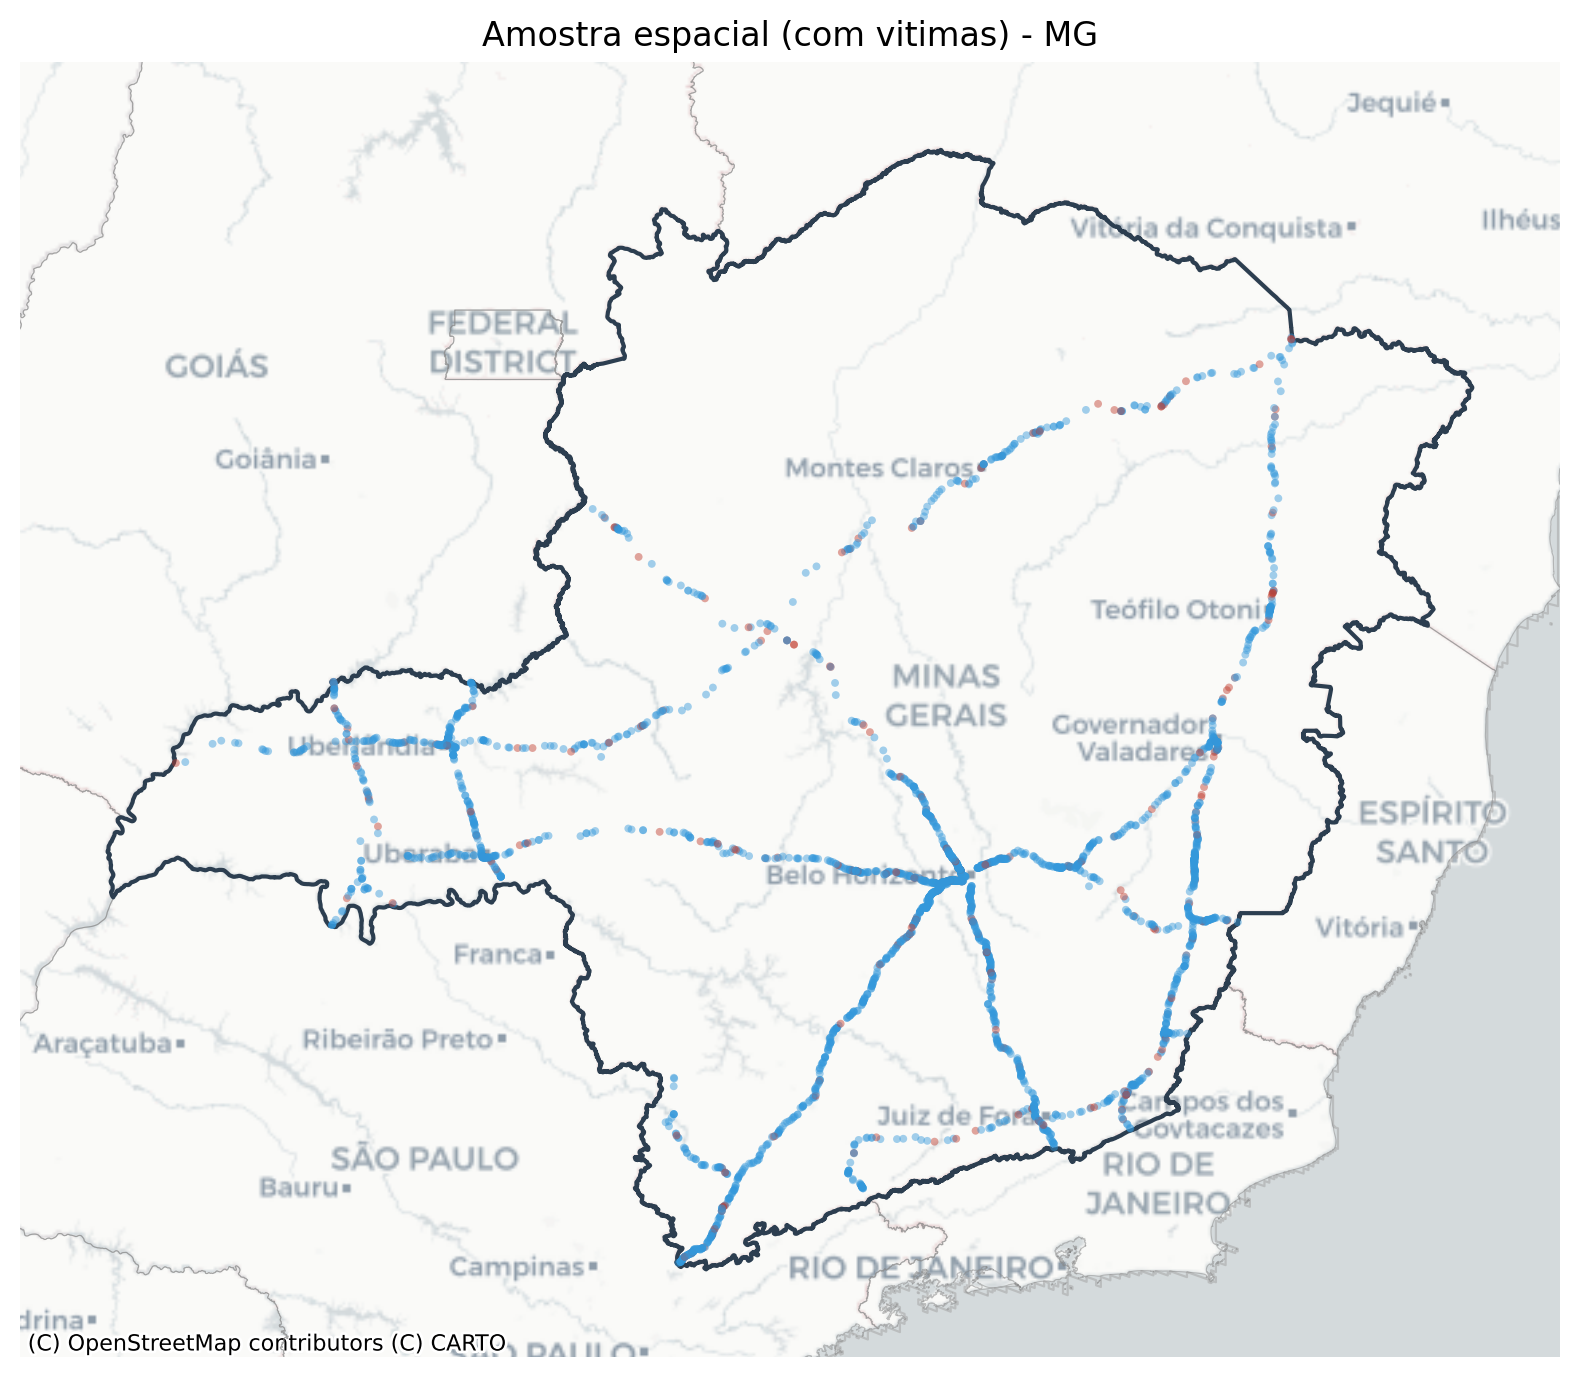
\includegraphics[width=\linewidth,height=12cm,keepaspectratio]{02_mapa_amostra.png}
        \fcap{A amostra cobre todo o estado, concentrando-se nas BRs e na Grande BH.}
      \end{column}
      \begin{column}{0.51\linewidth}
        \centering
        
\includegraphics[width=\linewidth,height=8.1cm,keepaspectratio]{02_heatmap_temporal_gravidade.png}
        \fcap{A severidade varia por fase do dia e dia da semana; noite e madrugada aparecem em perfis críticos.}

        \vspace{0.6ex}
        \raggedright
        \textbf{Por que MG?} O estado conecta fluxos entre \textbf{São Paulo, Rio de
        Janeiro, Espírito Santo, Bahia e Centro-Oeste}. Esse tráfego intenso e misto
        torna útil caracterizar perfis recorrentes de severidade.
      \end{column}
    \end{columns}

    \vspace{0.3ex}
    O recorte espaço-temporal orienta a leitura das regras: os padrões descrevem
    \textbf{severidade entre acidentes registrados}, não exposição total ao risco viário.

  \end{block}

  \begin{block}{4. Alvo e fatores associados}

    Antes de minerar regras, medimos a associação de cada variável com o alvo por
    Cramér's~$V$. Alta gravidade é menos rara que fatalidade pura, mas ainda representa
    os acidentes de maior impacto humano.

    \begin{columns}[c,totalwidth=\linewidth]
      \begin{column}{0.47\linewidth}
        \centering
        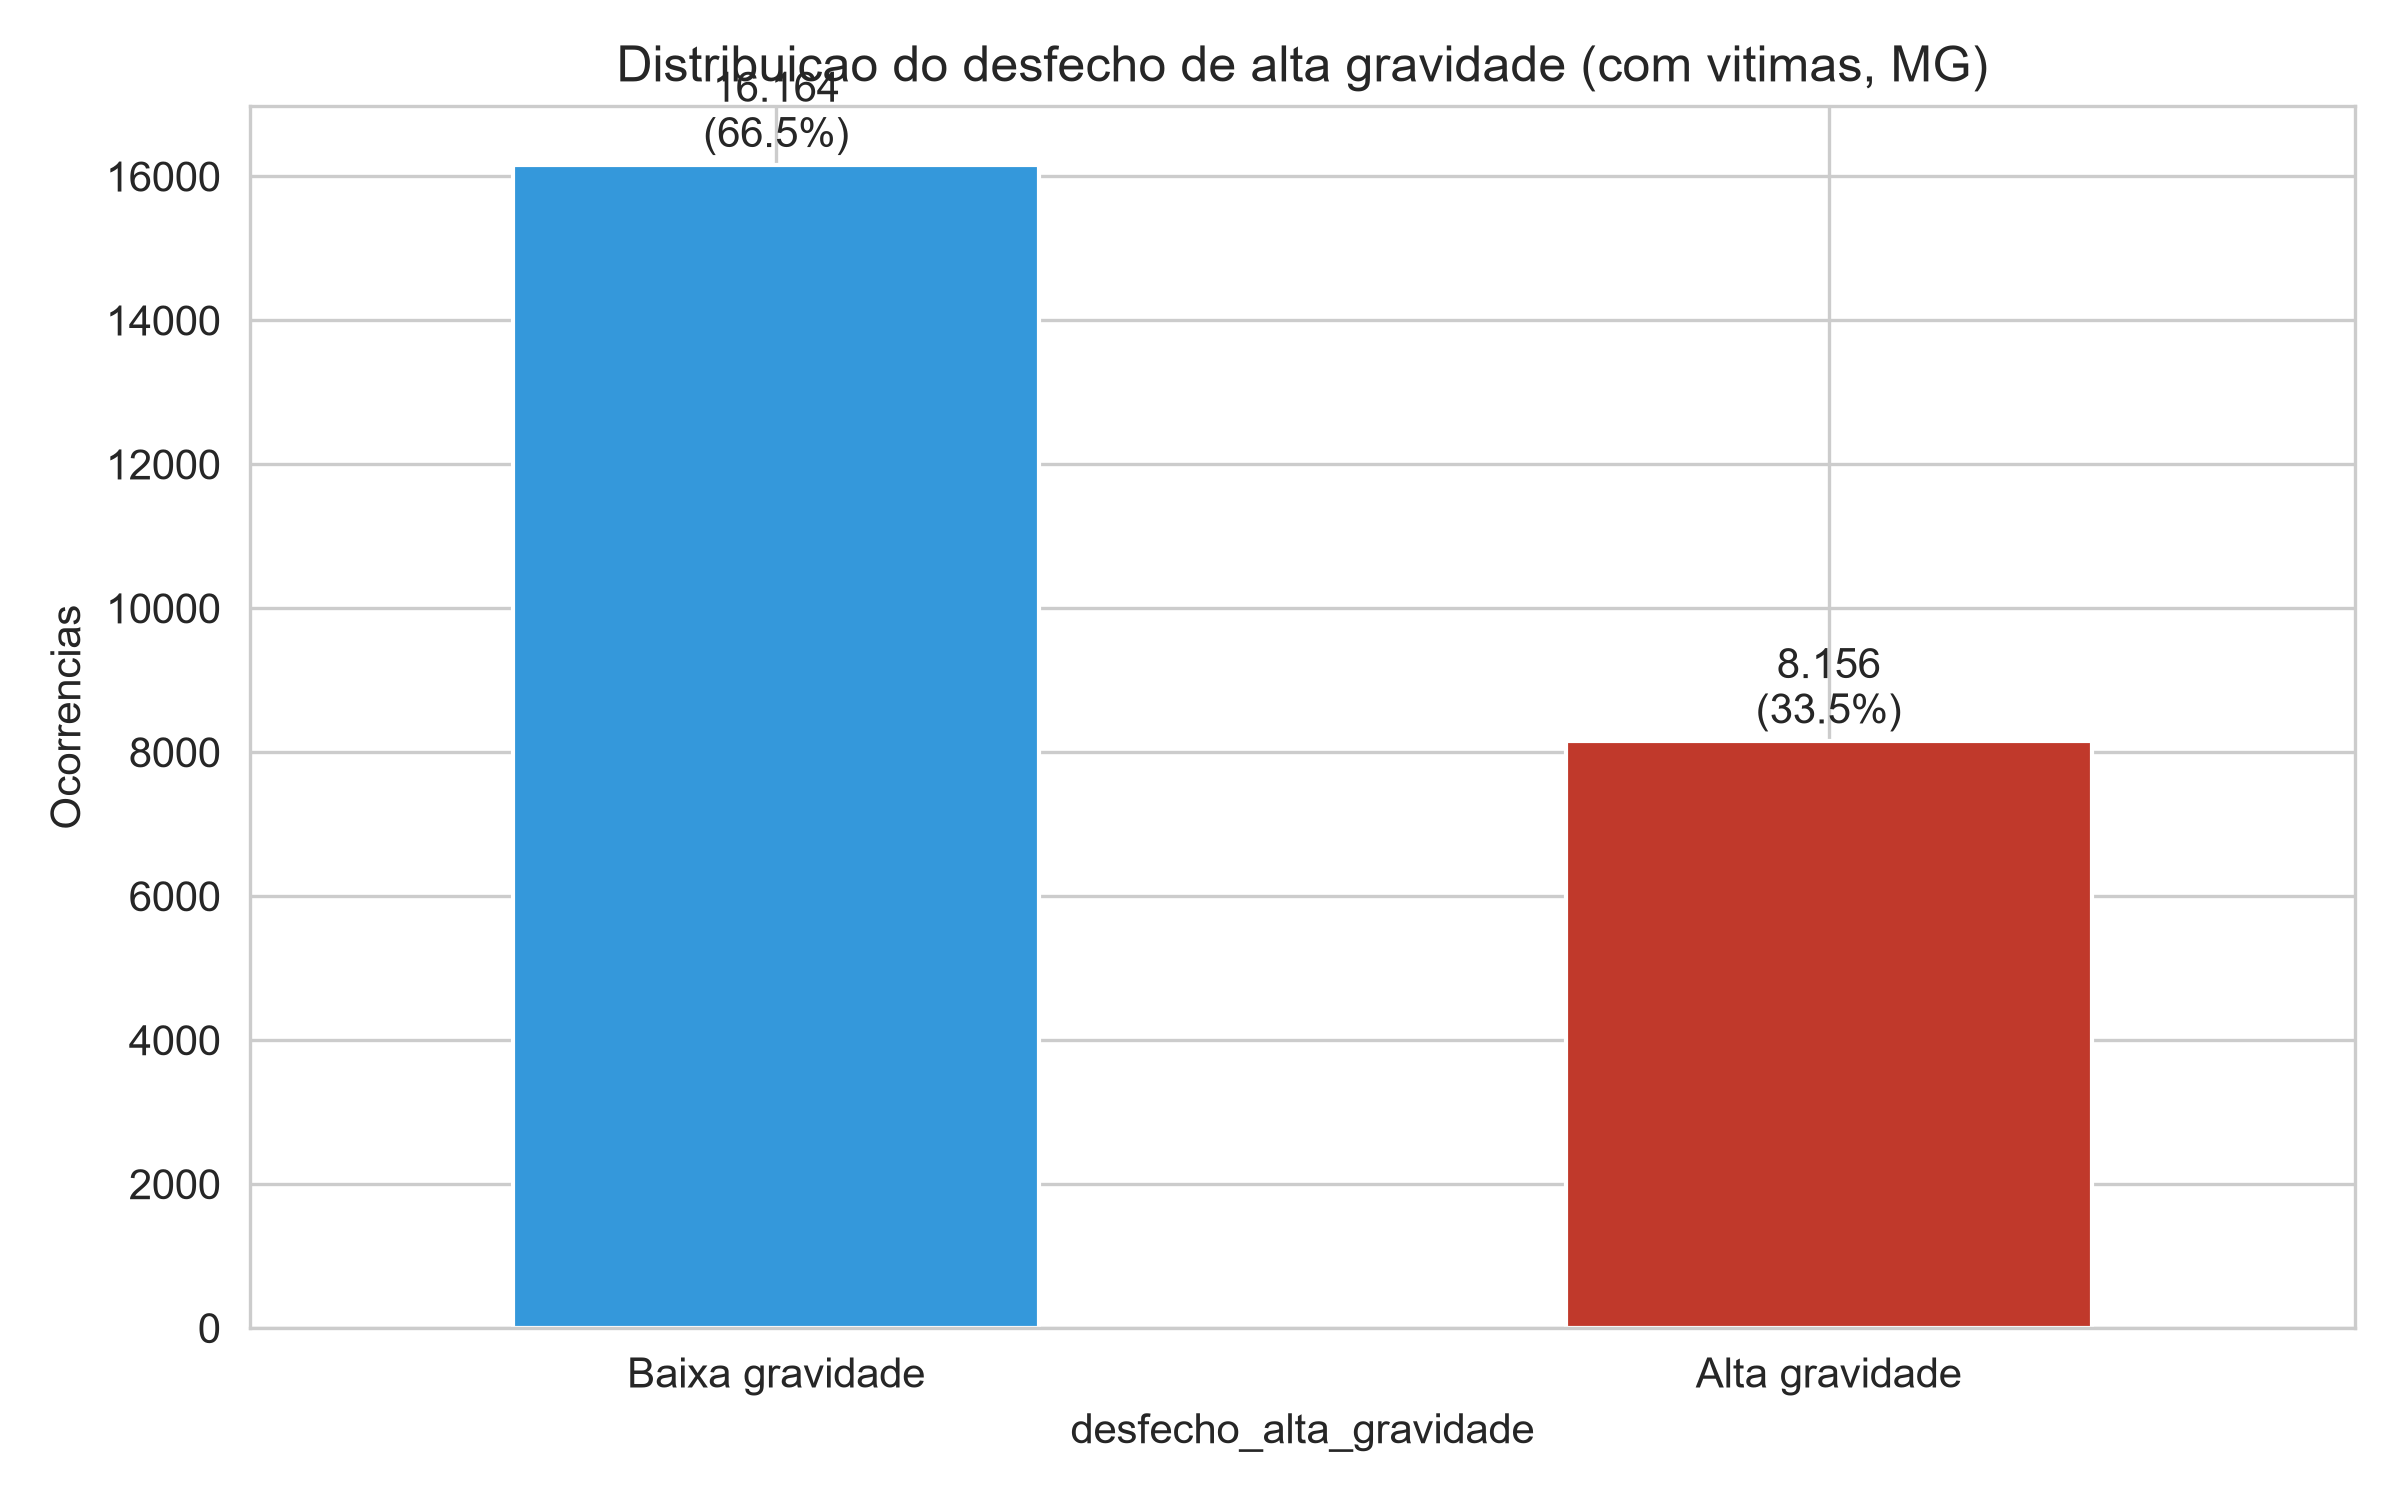
\includegraphics[width=\linewidth,height=7.5cm,keepaspectratio]{01_distribuicao_desfecho.png}
        \fcap{\textbf{33,54\%} das ocorrências com vítimas têm morto ou ferido grave.}
      \end{column}
      \begin{column}{0.50\linewidth}
        \centering
        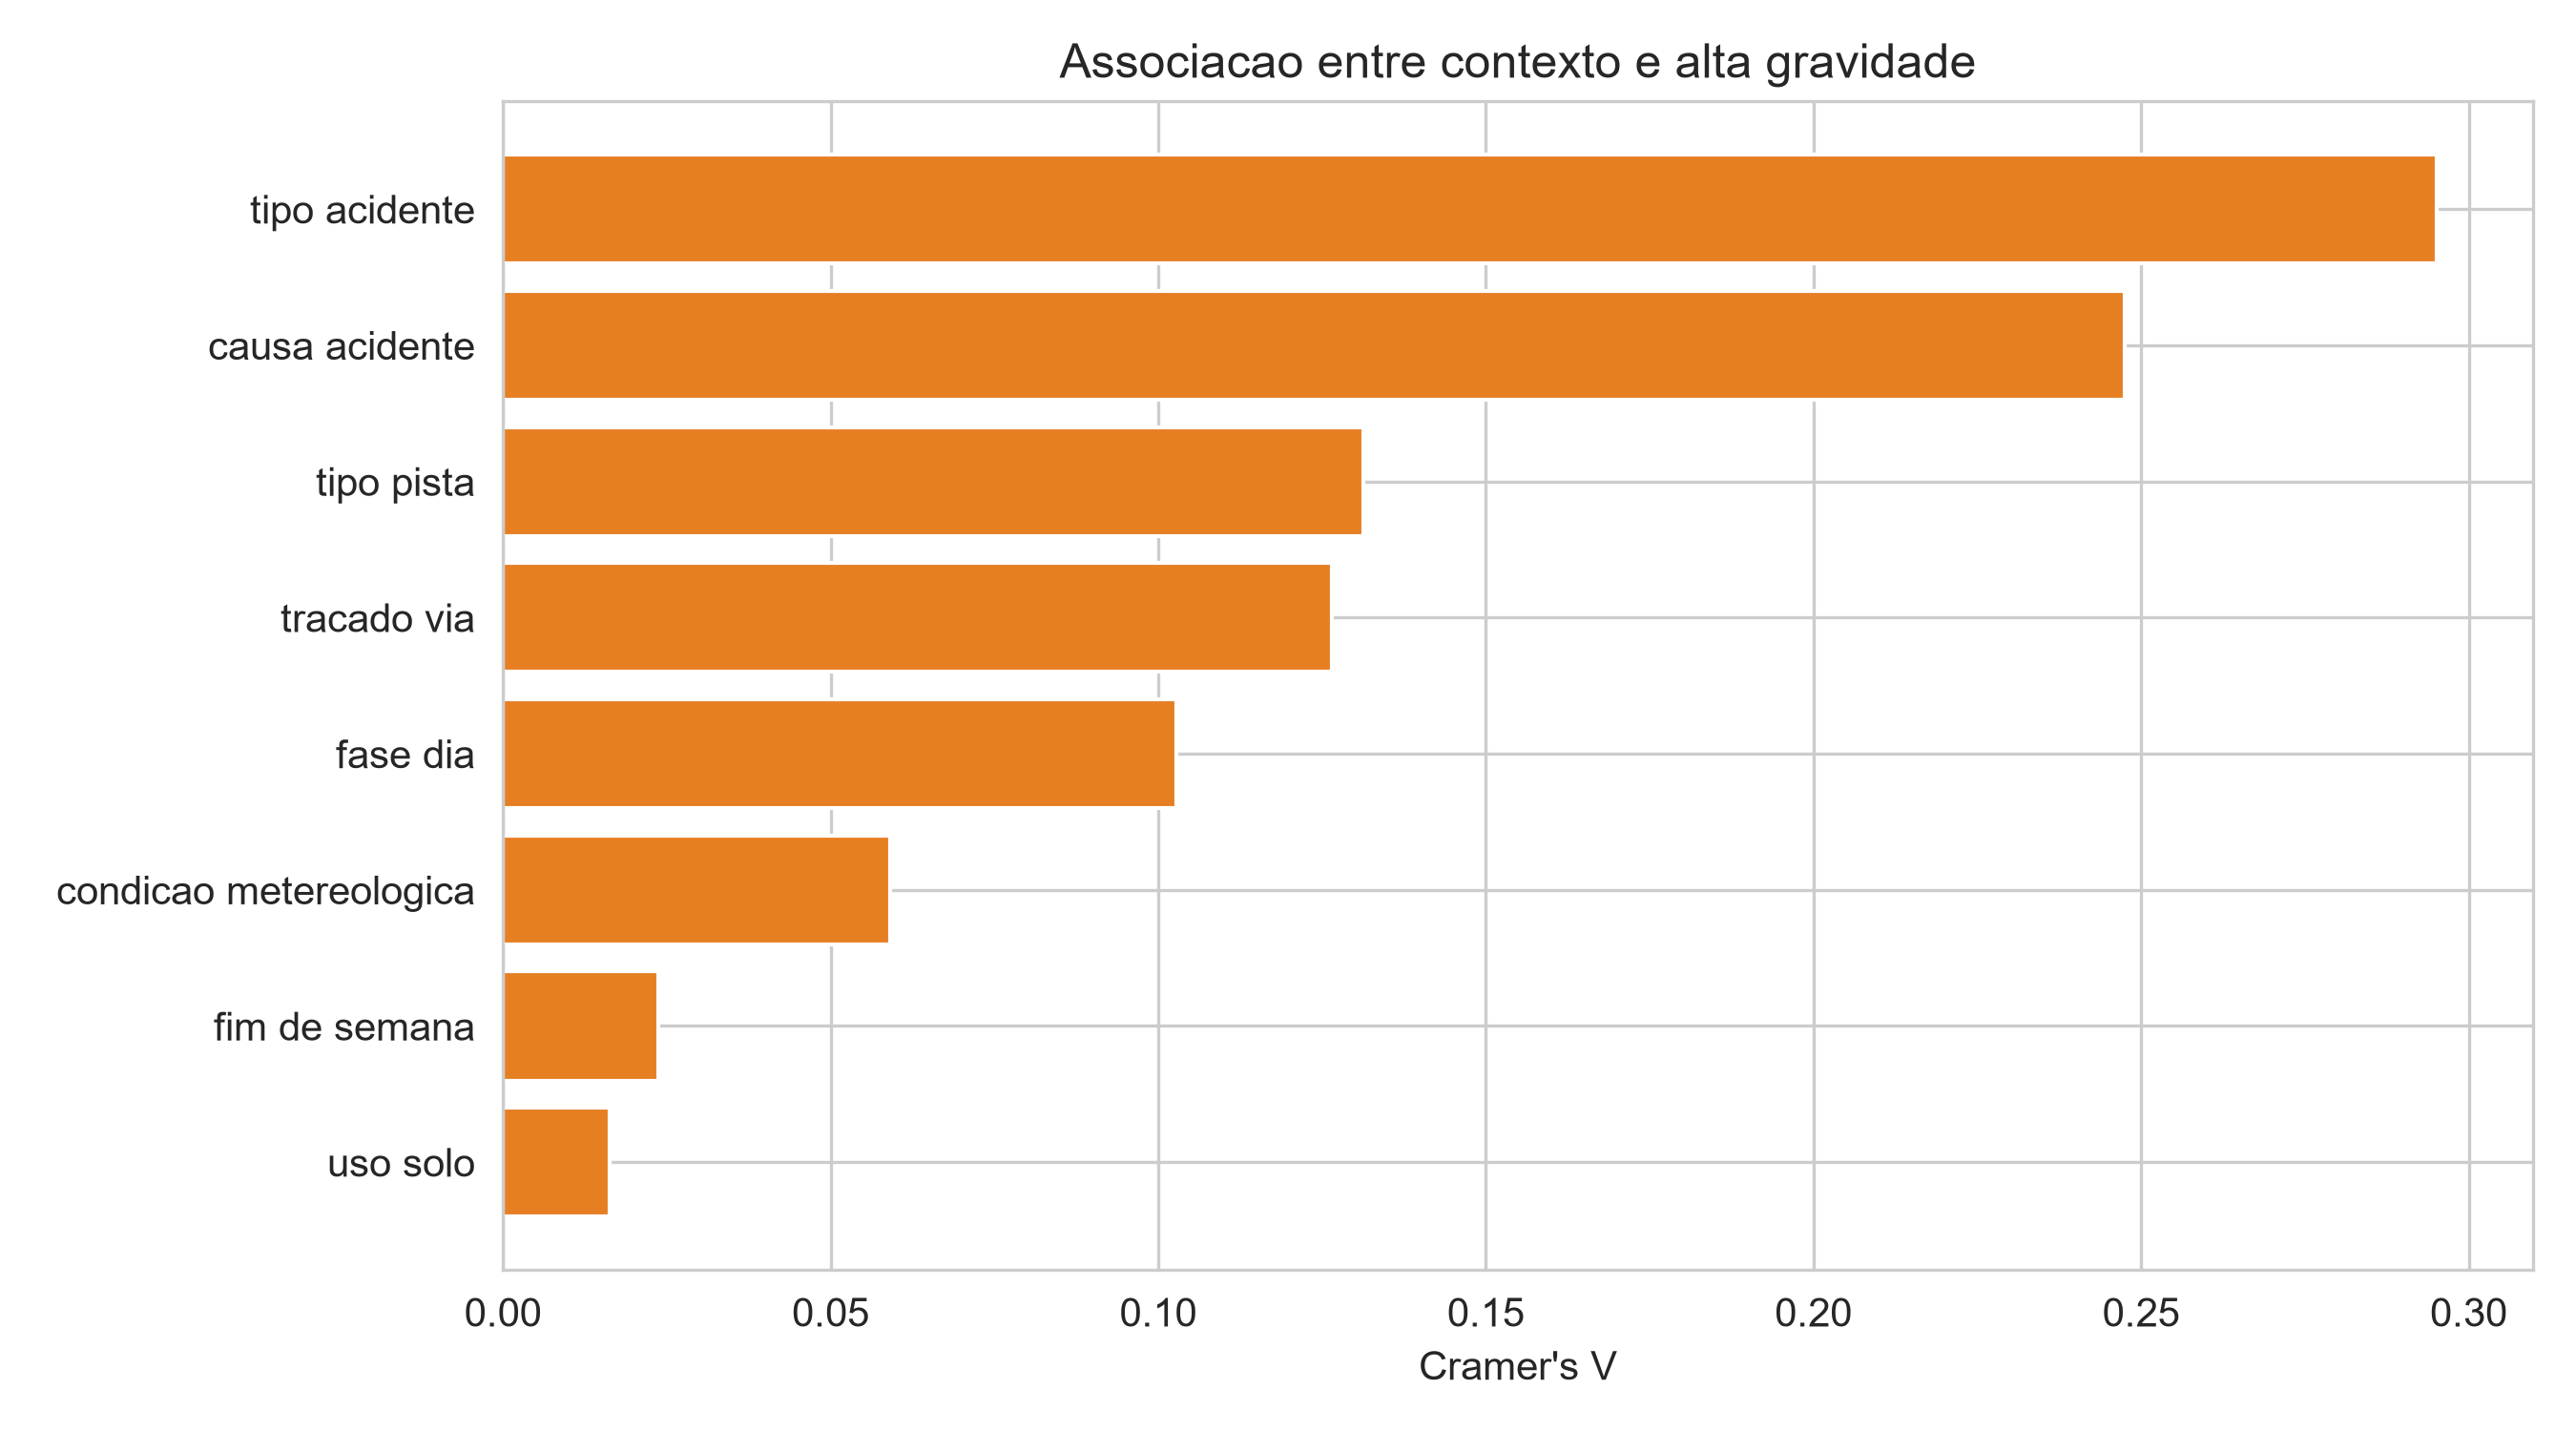
\includegraphics[width=\linewidth,height=7.5cm,keepaspectratio]{02_cramers_v_desfecho.png}
        \fcap{\textbf{Tipo} e \textbf{causa} da ocorrência lideram a associação com alta gravidade.}
      \end{column}
    \end{columns}

  \end{block}

\end{column}

\separatorcolumn

% ===================== COLUNA DIREITA =====================
\begin{column}{\colwidth}

  \begin{block}{5. As regras encontradas: perfis que multiplicam a severidade}

    As \textbf{154 regras} condensam combinações associadas à alta gravidade. As cinco
    principais (ordenadas por \emph{lift}) são:

    \vspace{0.9ex}
    \begin{center}
      \renewcommand{\arraystretch}{1.5}
      \small
      \setlength{\tabcolsep}{10pt}
      \begin{tabular}{@{}>{\raggedright\arraybackslash}p{12.8cm}rrr@{}}
        \toprule
        \textbf{Perfil da ocorrência} & \textbf{Sup.} & \textbf{Conf.} & \textbf{Lift} \\
        \midrule
        Pedestre na pista + Plena Noite + Atropelamento de pedestre & 0,6\% & 81,6\% & \hl{2,43} \\
        Pedestre na pista + Atropelamento de pedestre + Rural & 0,6\% & 80,9\% & \hl{2,41} \\
        Plena Noite + Atropelamento de pedestre + Rural & 1,0\% & 80,5\% & 2,40 \\
        Pedestre na pista + Plena Noite & 0,6\% & 80,3\% & 2,39 \\
        Pedestre na pista + Atropelamento de pedestre + Reta & 0,5\% & 80,0\% & 2,39 \\
        \bottomrule
      \end{tabular}
    \end{center}

    \heading{O que essas regras dizem}
    \begin{itemize}
      \item \textbf{Atropelamentos noturnos:} pedestres expostos, condições potencialmente
        associadas a menor visibilidade e dinâmica de impacto caracterizam o perfil mais
        severo.
      \item \textbf{Contramão e colisão frontal:} impactos de alta energia permanecem entre
        os padrões fortes, especialmente em análises de robustez.
      \item A contribuição não é causal: é \textbf{quantificar} força, cobertura,
        estabilidade e incerteza de padrões recorrentes.
    \end{itemize}

  \end{block}

  \begin{block}{6. Especificidade e cobertura dos perfis}

    \textit{Os perfis aparecem em qualquer acidente ou nos mais severos?} Avaliamos os
    mesmos antecedentes contra \textbf{BaixaGravidade} e \textbf{Fatal}. Quando o lift para
    alta gravidade fica perto de 2,4, o lift para baixa gravidade fica perto de 0,3; para
    fatalidade, vários perfis passam de 5. Assim, as regras são específicas de severidade.

    \vspace{0.6ex}
    \begin{columns}[c,totalwidth=\linewidth]
      \begin{column}{0.60\linewidth}
        \centering
        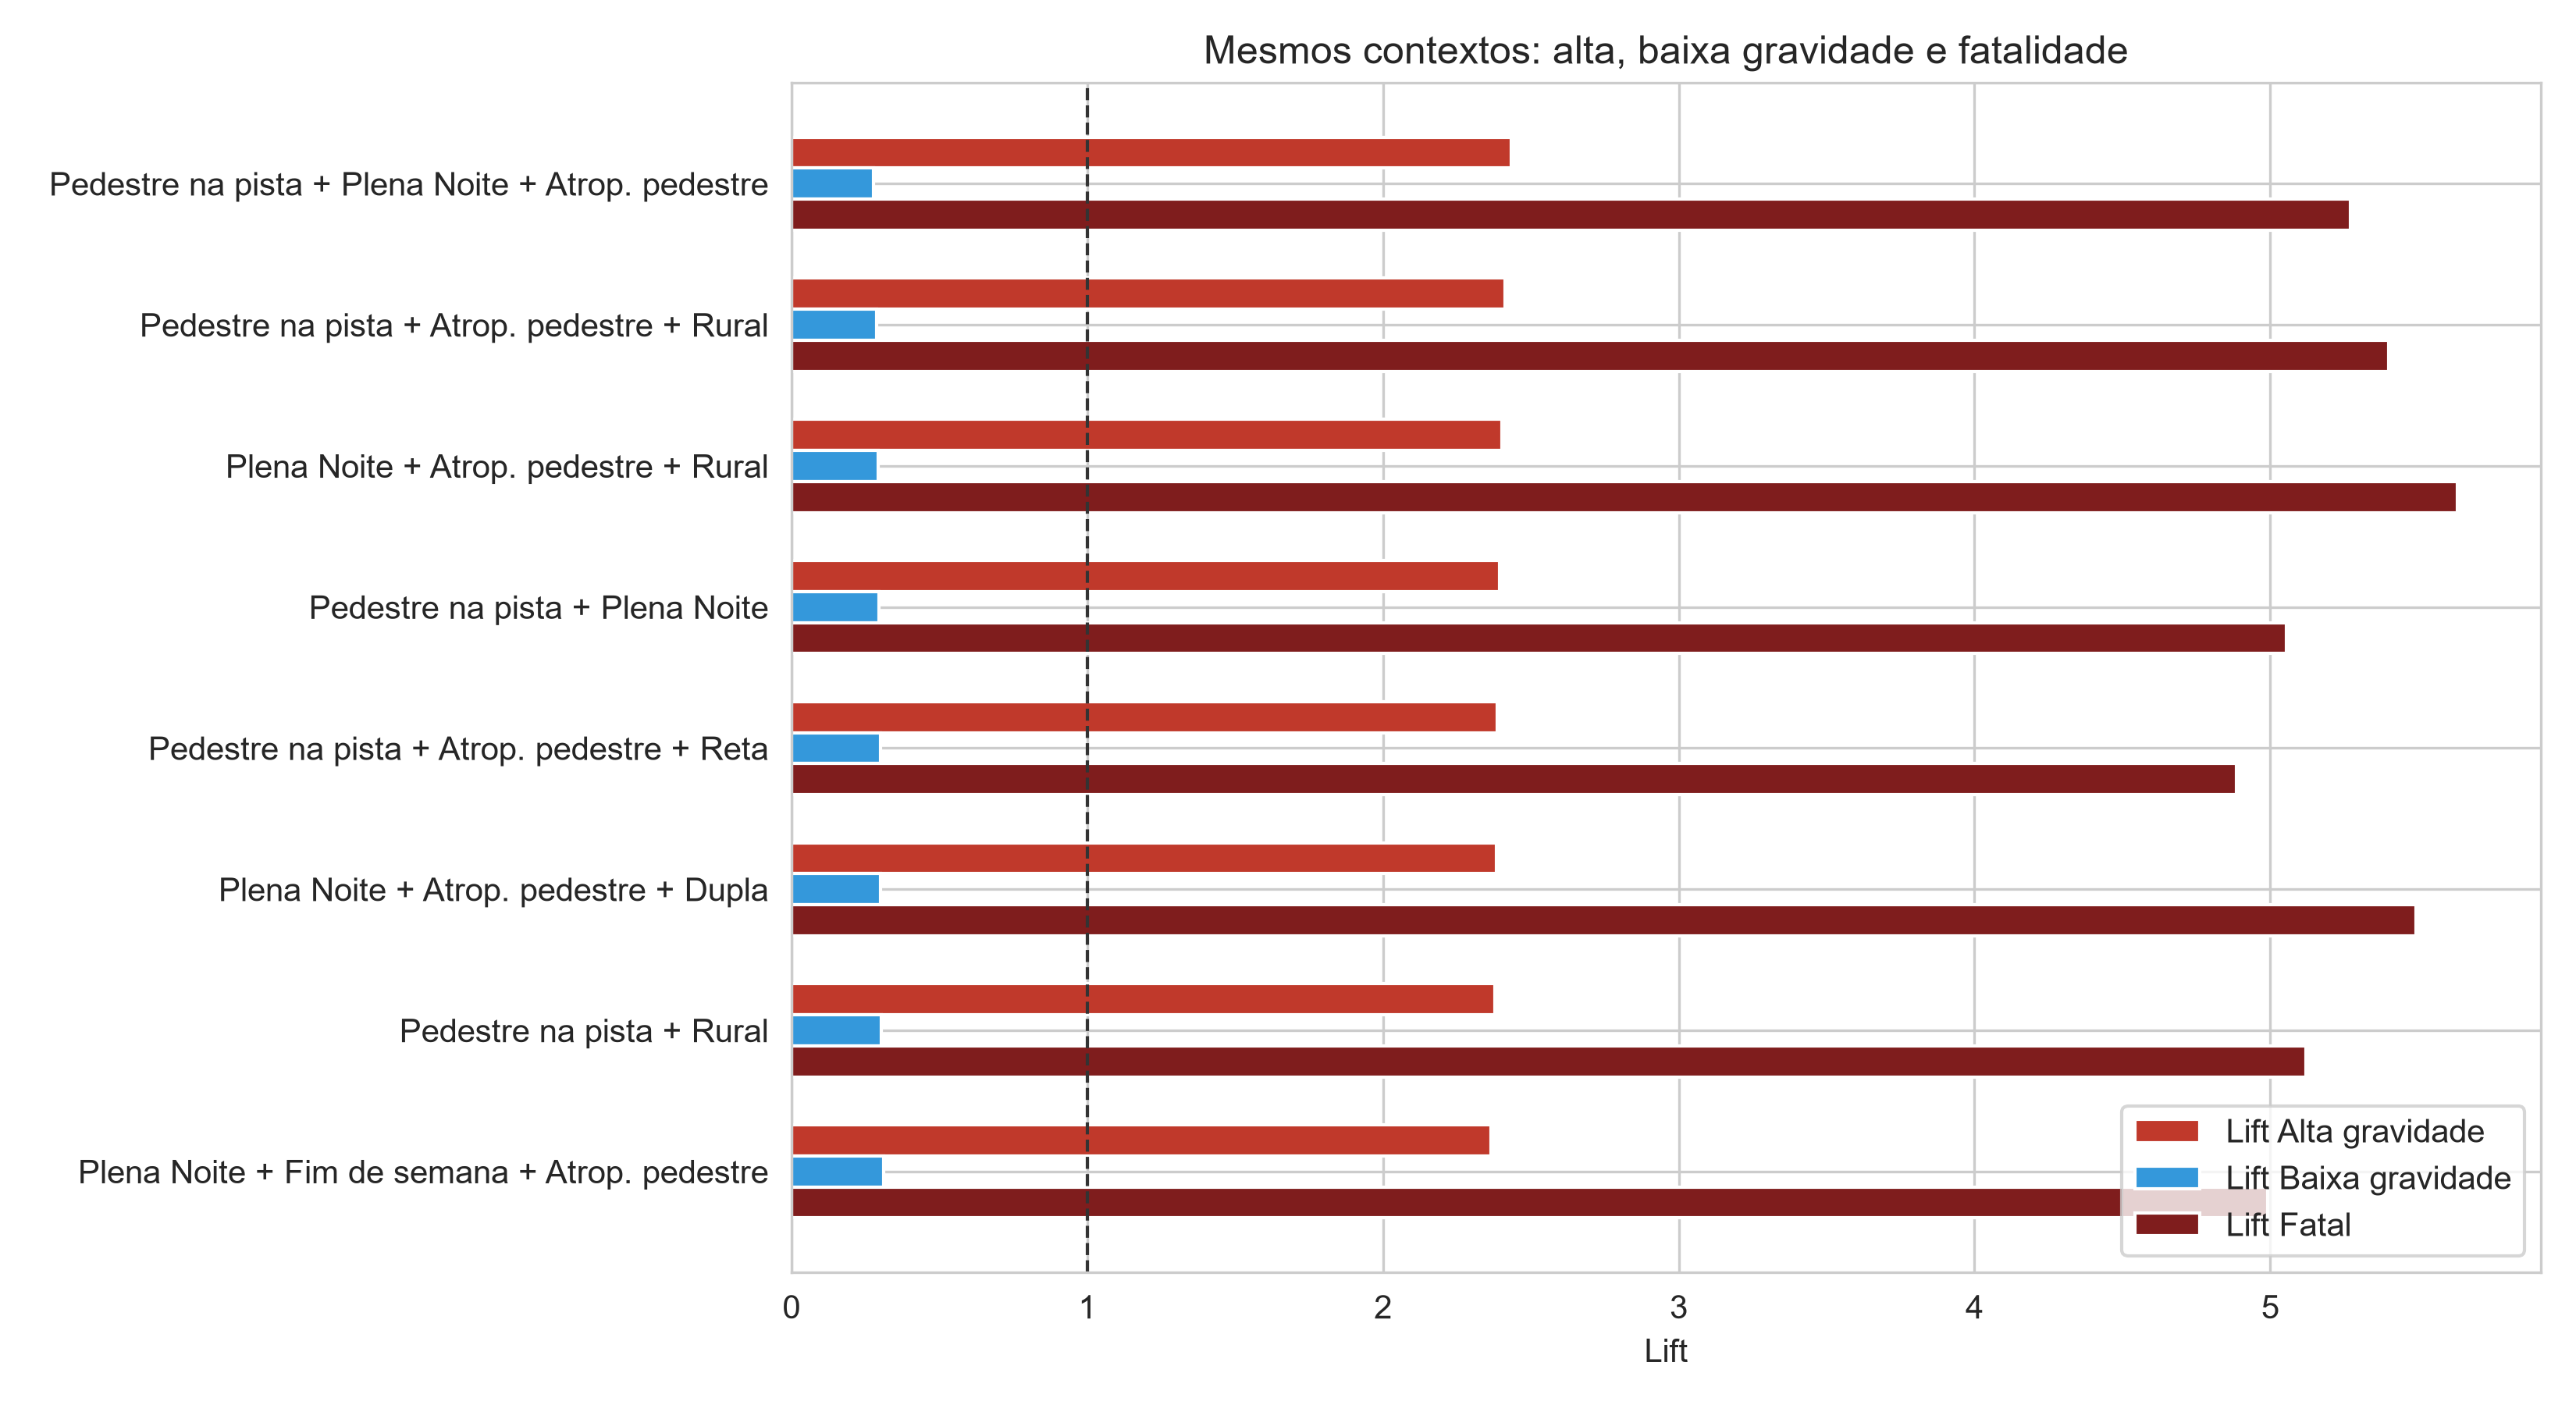
\includegraphics[width=\linewidth,height=9.2cm,keepaspectratio]{09_comparacao_alta_baixa_fatal.png}
        \fcap{Mesmos perfis: lift alto para Alta e Fatal, baixo para BaixaGravidade.}
      \end{column}
      \begin{column}{0.38\linewidth}
        \centering
        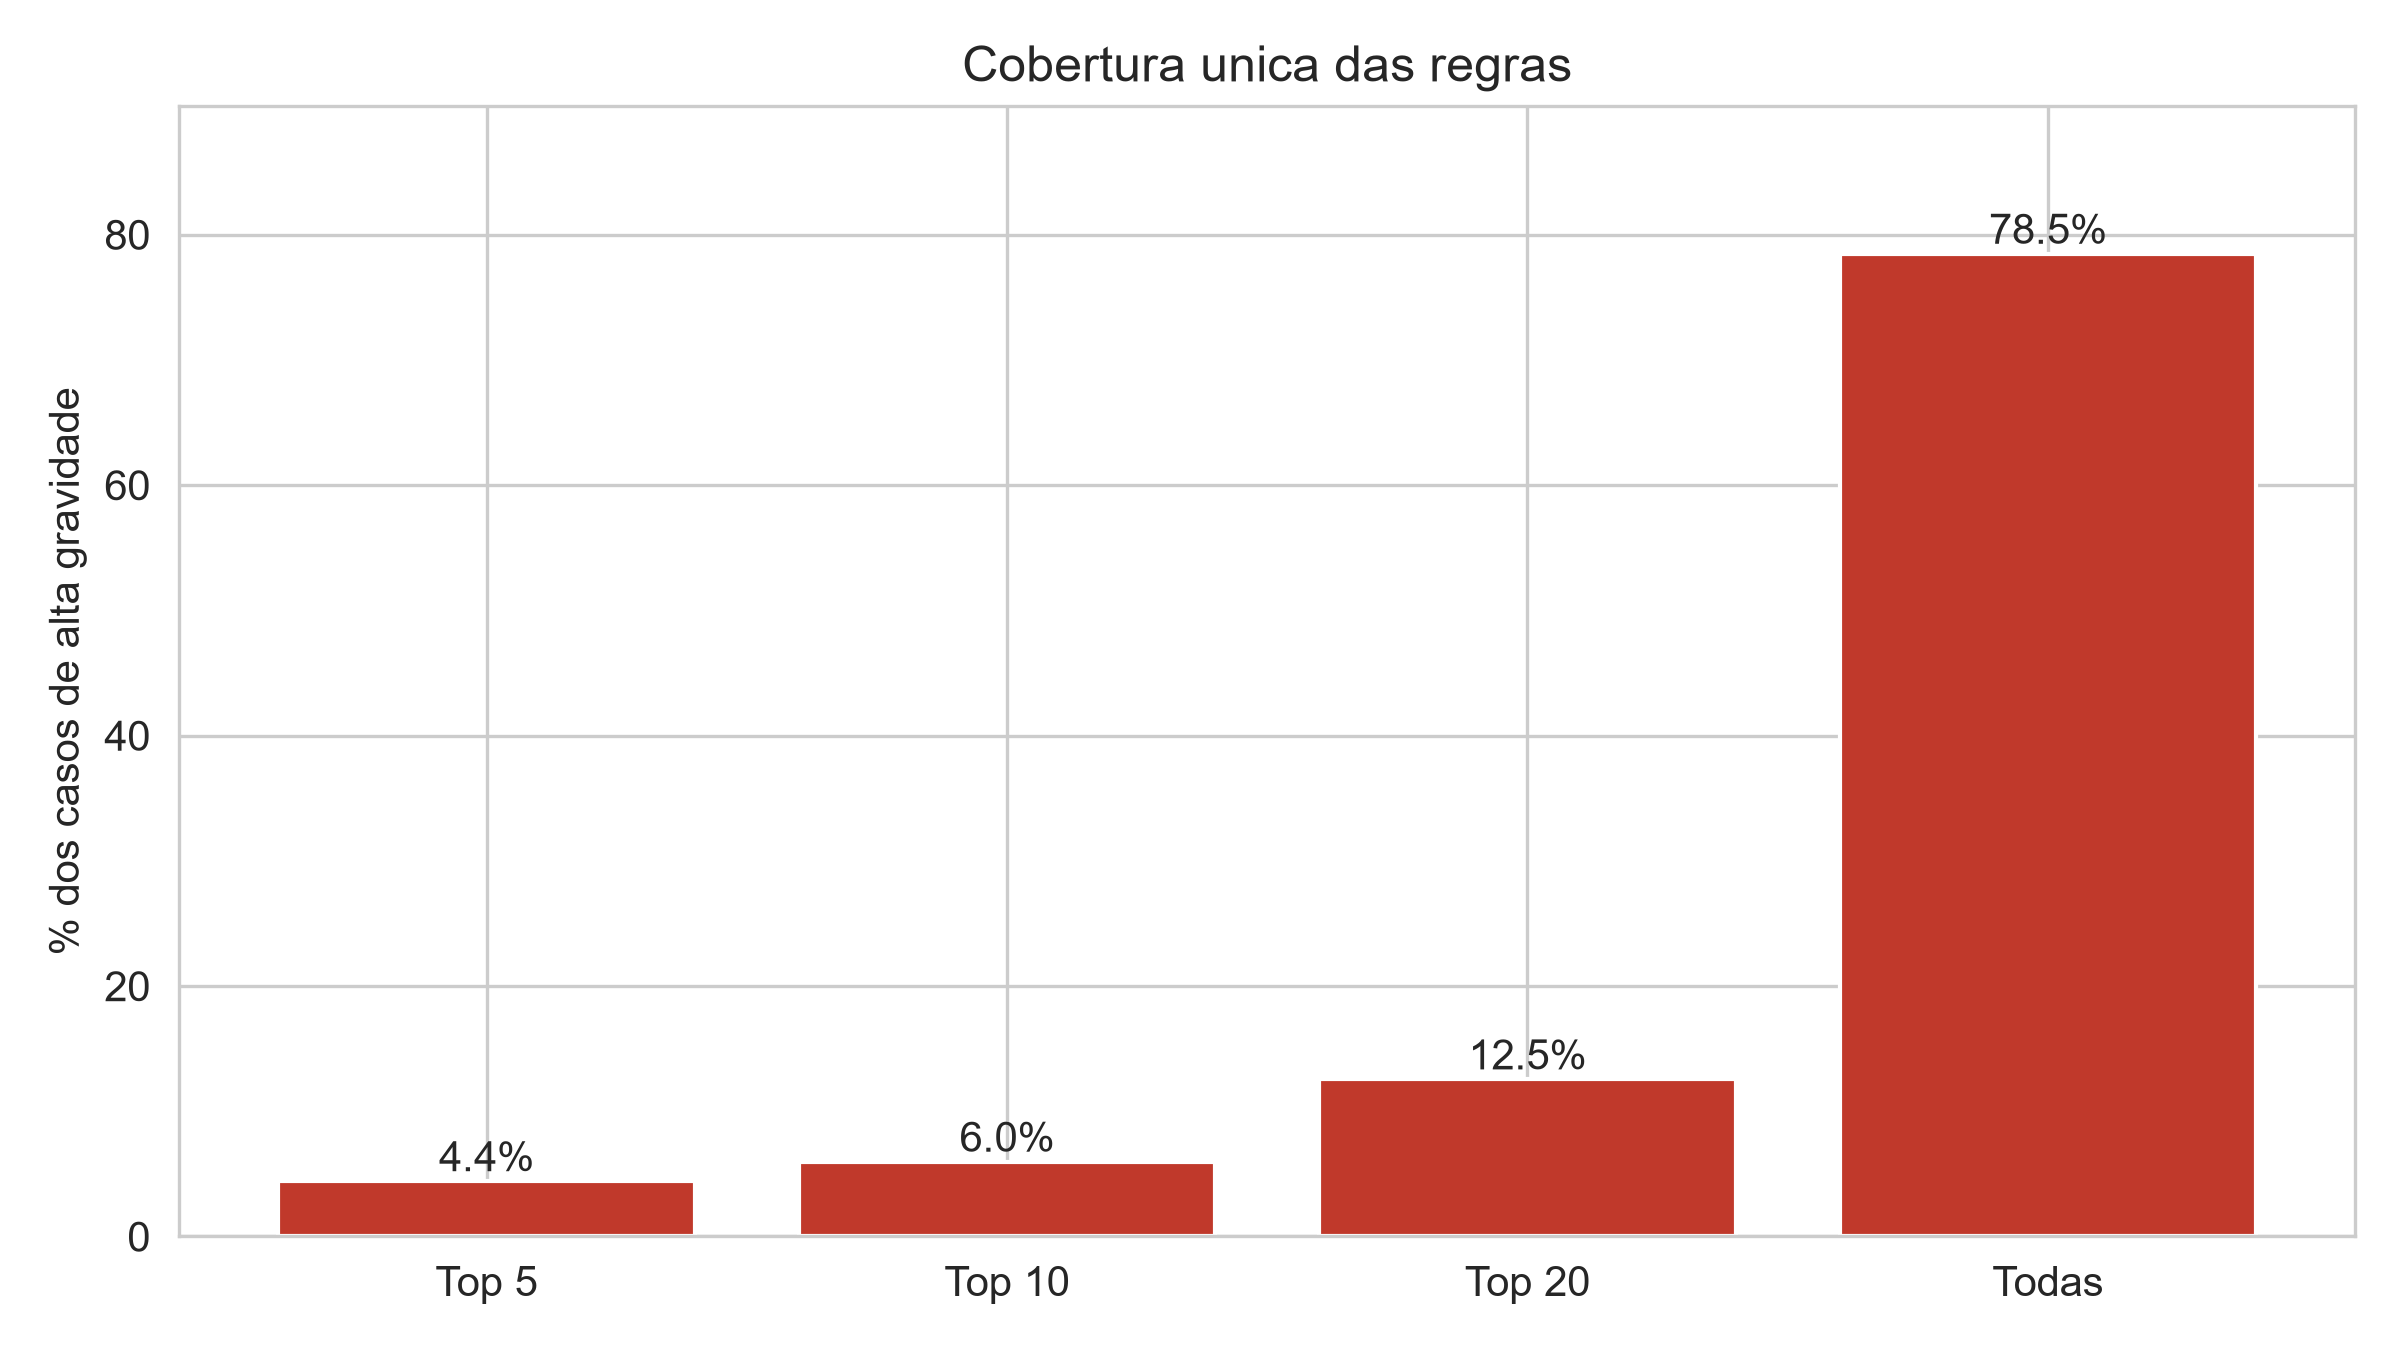
\includegraphics[width=\linewidth,height=8.3cm,keepaspectratio]{10_cobertura_regras.png}
        \fcap{Cobertura única dos perfis minerados.}
      \end{column}
    \end{columns}

    \vspace{0.5ex}
    \begin{itemize}
      \item \textbf{Top-5}: 360 casos severos cobertos; \textbf{Top-20}: 1.023.
      \item Todas as regras cobrem \textbf{78,5\%} dos casos severos, com menor seletividade.
      \item Há trade-off entre perfis muito fortes e cobertura operacional.
    \end{itemize}

  \end{block}

  \begin{block}{7. Robustez temporal, ambiente e incerteza}

    Minerando os anos completos separadamente, encontramos \hl{142 regras estáveis} (em
    pelo menos 2 de 3 anos) e \hl{60} presentes em \textbf{2023, 2024 e 2025}. A validação
    Jan--Abr inclui 2026 sem tratá-lo como ano completo. Por \textit{uso do solo}, há
    \textbf{112} regras urbanas e \textbf{122} rurais, com \texttt{uso\_solo} removido dos
    antecedentes.

    \begin{columns}[c,totalwidth=\linewidth]
      \begin{column}{0.5\linewidth}
        \centering
        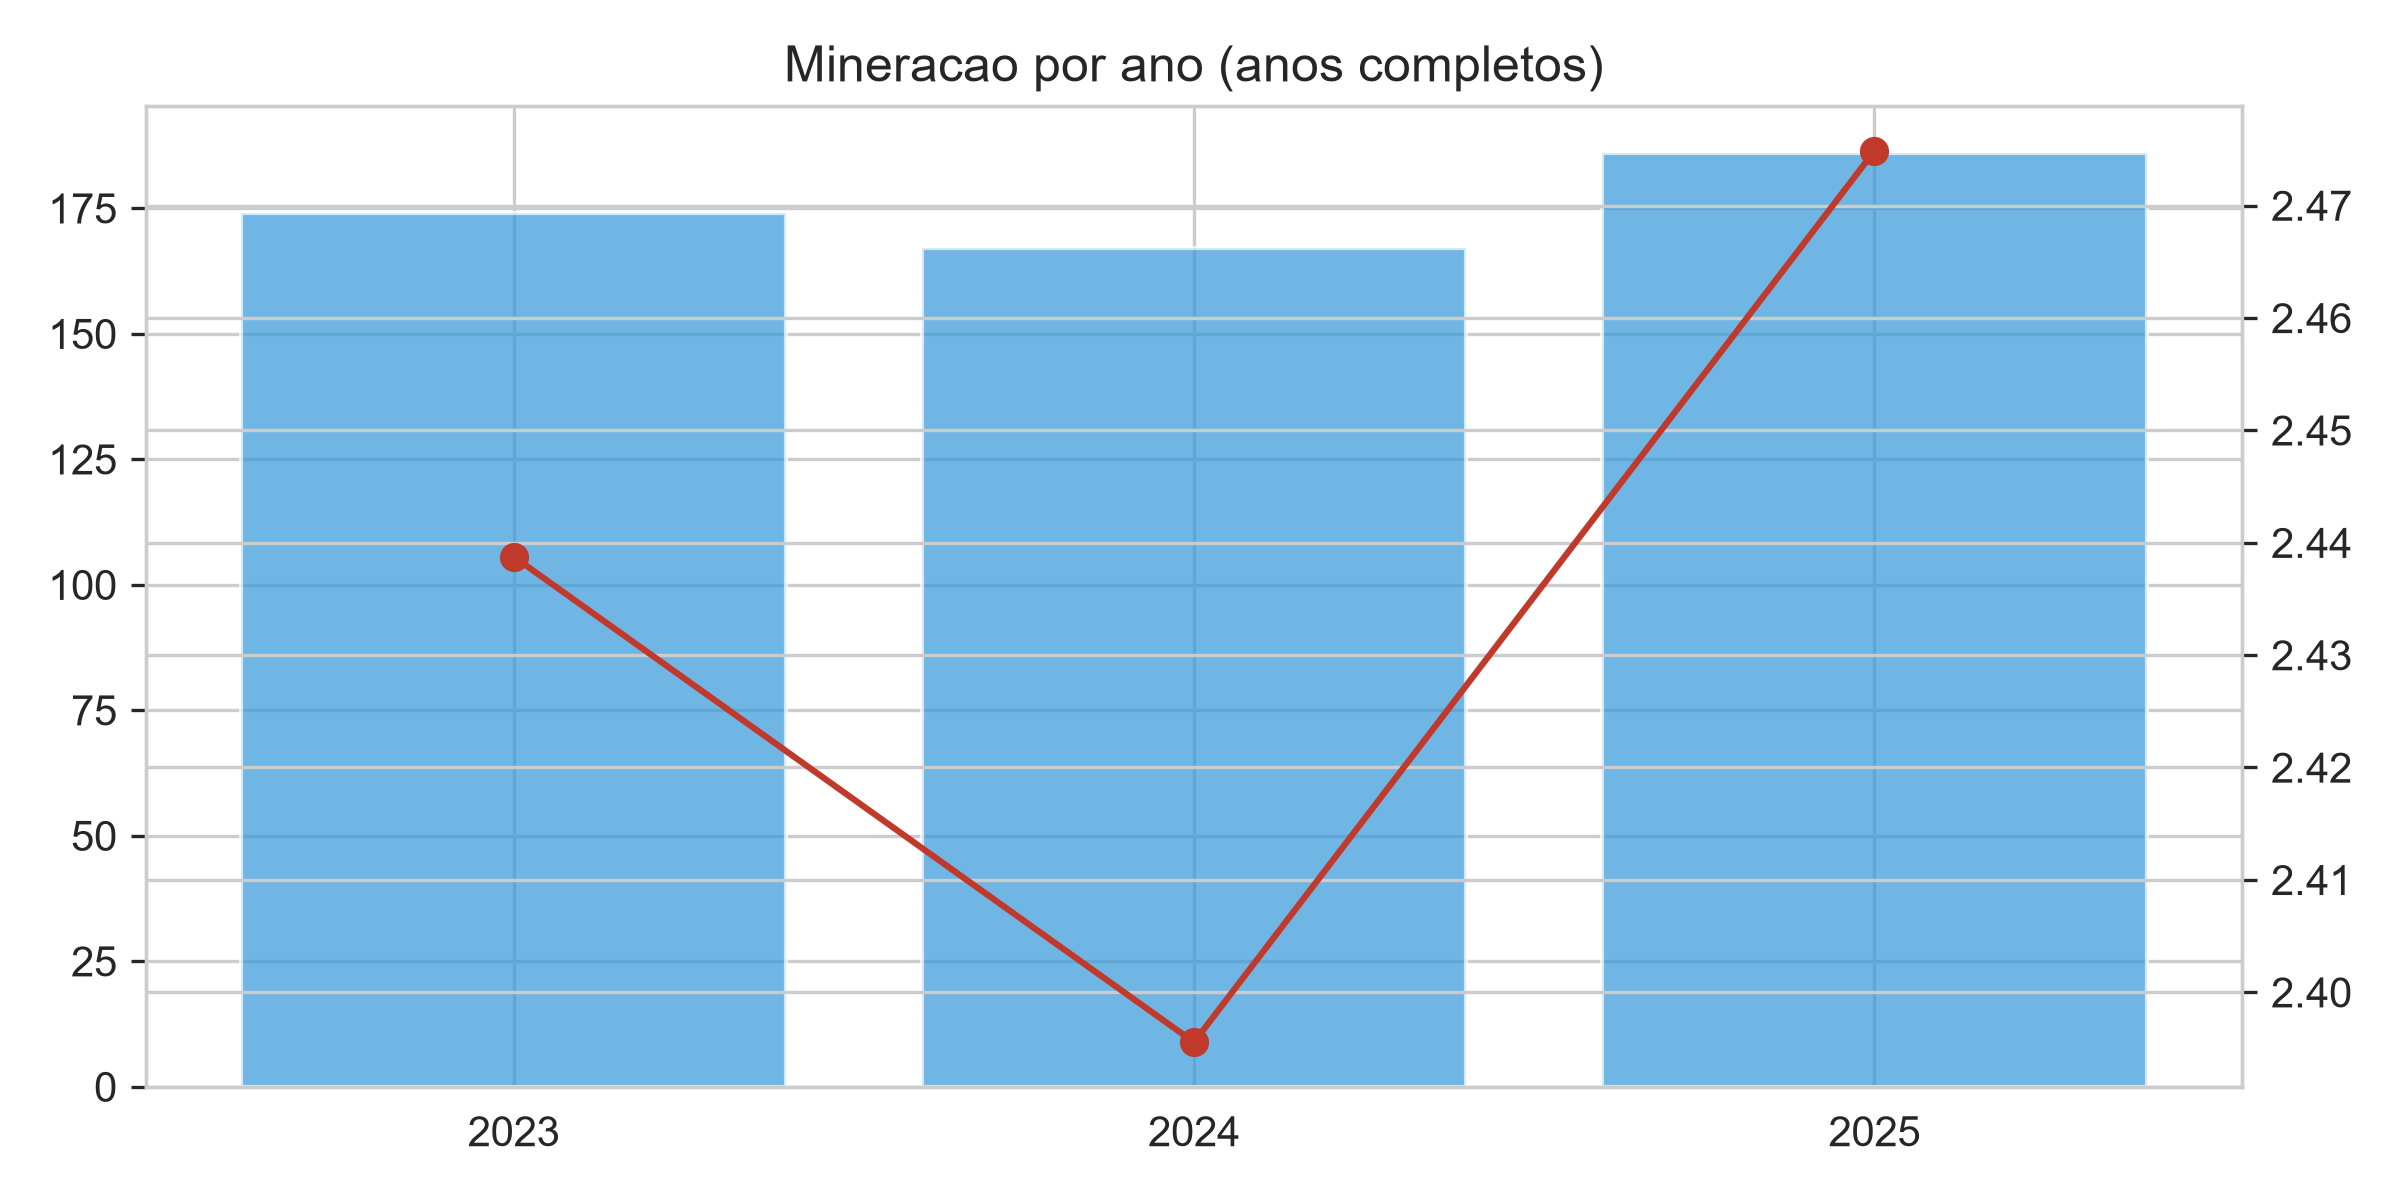
\includegraphics[width=\linewidth,height=6.4cm,keepaspectratio]{08_mineracao_por_ano.png}
        \fcap{Regras por ano e lift médio nos anos completos.}
      \end{column}
      \begin{column}{0.48\linewidth}
        \centering
        
\includegraphics[width=\linewidth,height=6.4cm,keepaspectratio]{07_estratos_uso_solo.png}
        \fcap{Perfis variam entre urbano e rural sem vazamento do estrato.}
      \end{column}
    \end{columns}

    \vspace{0.4ex}
    \textbf{Incerteza:} bootstrap com 400 reamostragens nas top-5 manteve lift IC95\% acima
    de \hl{2,19}. A sensibilidade de limiares preservou os perfis principais, embora o
    número de regras varie com suporte e confiança.

  \end{block}

  \begin{block}{8. Impacto, hipóteses e conclusões}

    \heading{O que cada hipótese revelou}
    \begin{columns}[T,totalwidth=\linewidth]
      \begin{column}{0.5\linewidth}
        \begin{itemize}
          \item \textbf{H3 -- tipo de acidente (confirmada como perfil):} atropelamentos e
            colisões frontais lideram a severidade.
          \item \textbf{H5 -- ambiente (confirmada):} urbano e rural têm padrões distintos.
          \item \textbf{H1 -- noite + perfil (parcial):} a noite importa sobretudo
            combinada a atropelamento ou colisão frontal.
        \end{itemize}
      \end{column}
      \begin{column}{0.46\linewidth}
        \begin{itemize}
          \item \textbf{H2 -- fim de semana (parcial):} aparece em alguns perfis, mas não
            domina isoladamente.
          \item \textbf{H4 -- clima adverso (não confirmada):} clima não aparece como fator
            dominante nas regras de maior lift.
        \end{itemize}
        \textbf{IA responsável:} regras curtas e traduzidas (\textbf{explicabilidade}) e
        avaliadas por estabilidade temporal, cobertura e bootstrap (\textbf{avaliação}).
      \end{column}
    \end{columns}

    \vspace{0.3ex}
    \heading{Conclusão}
    A mineração condensou \textbf{24.320 ocorrências com vítimas} em perfis claros,
    estáveis e específicos de alta gravidade. Os principais padrões envolvem
    \textbf{atropelamentos noturnos}, \textbf{pedestres na pista}, \textbf{contramão} e
    \textbf{colisões frontais}. A leitura correta é investigativa: as regras ajudam a
    priorizar hipóteses de prevenção, mas \hl{associação não é causalidade} e o estudo não
    estima risco absoluto de ocorrência.

  \end{block}

\end{column}
\separatorcolumn
\end{columns}
\end{frame}

\end{document}
